% Options for packages loaded elsewhere
\PassOptionsToPackage{unicode}{hyperref}
\PassOptionsToPackage{hyphens}{url}
\PassOptionsToPackage{dvipsnames,svgnames,x11names}{xcolor}
%
\documentclass[
  a4paper,
  DIV=11,
  numbers=noendperiod]{scrartcl}

\usepackage{amsmath,amssymb}
\usepackage{iftex}
\ifPDFTeX
  \usepackage[T1]{fontenc}
  \usepackage[utf8]{inputenc}
  \usepackage{textcomp} % provide euro and other symbols
\else % if luatex or xetex
  \usepackage{unicode-math}
  \defaultfontfeatures{Scale=MatchLowercase}
  \defaultfontfeatures[\rmfamily]{Ligatures=TeX,Scale=1}
\fi
\usepackage{lmodern}
\ifPDFTeX\else  
    % xetex/luatex font selection
\fi
% Use upquote if available, for straight quotes in verbatim environments
\IfFileExists{upquote.sty}{\usepackage{upquote}}{}
\IfFileExists{microtype.sty}{% use microtype if available
  \usepackage[]{microtype}
  \UseMicrotypeSet[protrusion]{basicmath} % disable protrusion for tt fonts
}{}
\makeatletter
\@ifundefined{KOMAClassName}{% if non-KOMA class
  \IfFileExists{parskip.sty}{%
    \usepackage{parskip}
  }{% else
    \setlength{\parindent}{0pt}
    \setlength{\parskip}{6pt plus 2pt minus 1pt}}
}{% if KOMA class
  \KOMAoptions{parskip=half}}
\makeatother
\usepackage{xcolor}
\setlength{\emergencystretch}{3em} % prevent overfull lines
\setcounter{secnumdepth}{-\maxdimen} % remove section numbering
% Make \paragraph and \subparagraph free-standing
\ifx\paragraph\undefined\else
  \let\oldparagraph\paragraph
  \renewcommand{\paragraph}[1]{\oldparagraph{#1}\mbox{}}
\fi
\ifx\subparagraph\undefined\else
  \let\oldsubparagraph\subparagraph
  \renewcommand{\subparagraph}[1]{\oldsubparagraph{#1}\mbox{}}
\fi


\providecommand{\tightlist}{%
  \setlength{\itemsep}{0pt}\setlength{\parskip}{0pt}}\usepackage{longtable,booktabs,array}
\usepackage{calc} % for calculating minipage widths
% Correct order of tables after \paragraph or \subparagraph
\usepackage{etoolbox}
\makeatletter
\patchcmd\longtable{\par}{\if@noskipsec\mbox{}\fi\par}{}{}
\makeatother
% Allow footnotes in longtable head/foot
\IfFileExists{footnotehyper.sty}{\usepackage{footnotehyper}}{\usepackage{footnote}}
\makesavenoteenv{longtable}
\usepackage{graphicx}
\makeatletter
\def\maxwidth{\ifdim\Gin@nat@width>\linewidth\linewidth\else\Gin@nat@width\fi}
\def\maxheight{\ifdim\Gin@nat@height>\textheight\textheight\else\Gin@nat@height\fi}
\makeatother
% Scale images if necessary, so that they will not overflow the page
% margins by default, and it is still possible to overwrite the defaults
% using explicit options in \includegraphics[width, height, ...]{}
\setkeys{Gin}{width=\maxwidth,height=\maxheight,keepaspectratio}
% Set default figure placement to htbp
\makeatletter
\def\fps@figure{htbp}
\makeatother

\KOMAoption{captions}{tableheading}
\makeatletter
\@ifpackageloaded{caption}{}{\usepackage{caption}}
\AtBeginDocument{%
\ifdefined\contentsname
  \renewcommand*\contentsname{Table of contents}
\else
  \newcommand\contentsname{Table of contents}
\fi
\ifdefined\listfigurename
  \renewcommand*\listfigurename{List of Figures}
\else
  \newcommand\listfigurename{List of Figures}
\fi
\ifdefined\listtablename
  \renewcommand*\listtablename{List of Tables}
\else
  \newcommand\listtablename{List of Tables}
\fi
\ifdefined\figurename
  \renewcommand*\figurename{Figure}
\else
  \newcommand\figurename{Figure}
\fi
\ifdefined\tablename
  \renewcommand*\tablename{Table}
\else
  \newcommand\tablename{Table}
\fi
}
\@ifpackageloaded{float}{}{\usepackage{float}}
\floatstyle{ruled}
\@ifundefined{c@chapter}{\newfloat{codelisting}{h}{lop}}{\newfloat{codelisting}{h}{lop}[chapter]}
\floatname{codelisting}{Listing}
\newcommand*\listoflistings{\listof{codelisting}{List of Listings}}
\makeatother
\makeatletter
\makeatother
\makeatletter
\@ifpackageloaded{caption}{}{\usepackage{caption}}
\@ifpackageloaded{subcaption}{}{\usepackage{subcaption}}
\makeatother
\ifLuaTeX
  \usepackage{selnolig}  % disable illegal ligatures
\fi
\usepackage{bookmark}

\IfFileExists{xurl.sty}{\usepackage{xurl}}{} % add URL line breaks if available
\urlstyle{same} % disable monospaced font for URLs
\hypersetup{
  pdftitle={Definitie-fase},
  colorlinks=true,
  linkcolor={blue},
  filecolor={Maroon},
  citecolor={Blue},
  urlcolor={Blue},
  pdfcreator={LaTeX via pandoc}}

\title{Definitie-fase}
\author{}
\date{}

\begin{document}
\maketitle

\renewcommand*\contentsname{Table of contents}
{
\hypersetup{linkcolor=}
\setcounter{tocdepth}{3}
\tableofcontents
}
\listoffigures
\listoftables
Sinds 2,5 jaar geef ik les op de Hogeschool van Amsterdam (HvA) op de
Faculteit Business en Economie (FBE) binnen het cluster Finance \&
Control (F\&C). In dit hoofdstuk, de ``Define Fase'', ligt ik hieronder
eerst toe hoe ik gekomen ben tot het procesverbeter voorstel.

\subsection{Proces-selectie}\label{proces-selectie}

Mijn verzoek om de opdracht t.b.v. het Green Belt Certificaat te kunnen
doen is goedgekeurd door de Finance \& Control coördinator Nadine
Steverink. Met de goedkeuring kwam de vraag om een onderwerp te kiezen
dat te maken heeft met de opleiding. Ik had toen het idee om het project
te doen over een onderdeel van de opleiding waarin ik zelf actief ben.
Hierna heb ik mondeling overleg gehad met mijn collega's Gert de Jong en
Paul te Riele. De collega's stonden niet afwijzend tegenover het idee.
Ons regulier periodiek overleg geeft mij de gelegenheid om
terugkoppeling te vragen op de deelproducten van het project.

Hieronder is staat een generiek proces van een onderwijs module
weergegeven. Dit LSS project situeert zich in de processtap ``Het
uitvoeren van onderwijs''. Hieronder wordt verstaan het geven van
lessen, het begeleiden van studenten en het beoordelen van
leerresultaten.

\begin{figure}[H]

{\centering 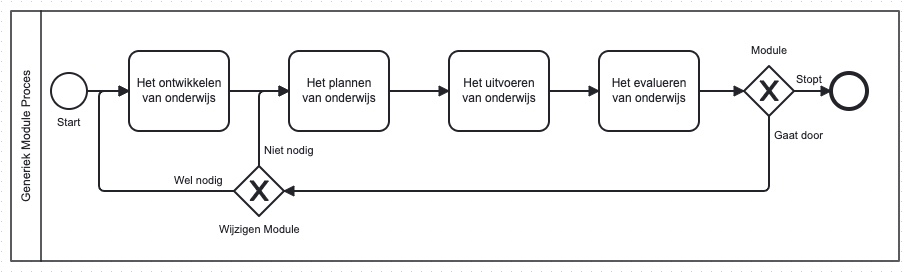
\includegraphics{./static/module_generiek.jpg}

}

\caption{Generiek Module Proces}

\end{figure}%

\newpage

\subsection{Project Charter}\label{project-charter}

Het project charter heeft als doel een éénduidige beschrijving van het
project te geven zodat betrokkenen het doel, de rijkwijdte en de
planning kennen. De werktitel van het project is ``verbeteren door
versnellen'' (van de e-learnings).

\begin{longtable}[]{@{}
  >{\raggedright\arraybackslash}p{(\columnwidth - 2\tabcolsep) * \real{0.4730}}
  >{\raggedright\arraybackslash}p{(\columnwidth - 2\tabcolsep) * \real{0.5270}}@{}}
\caption{Project Charter}\tabularnewline
\toprule\noalign{}
\begin{minipage}[b]{\linewidth}\raggedright
\textbf{Business Case}
\end{minipage} & \begin{minipage}[b]{\linewidth}\raggedright
\textbf{Scope}
\end{minipage} \\
\midrule\noalign{}
\endfirsthead
\toprule\noalign{}
\begin{minipage}[b]{\linewidth}\raggedright
\textbf{Business Case}
\end{minipage} & \begin{minipage}[b]{\linewidth}\raggedright
\textbf{Scope}
\end{minipage} \\
\midrule\noalign{}
\endhead
\bottomrule\noalign{}
\endlastfoot
& \\
Operations wordt, als vak binnen & Organisatie: Hogeschool van
Amsterdam \\
Processen \& Risico twee keer per & Faculteit: Business \& Economie \\
jaar gegeven. Aanname is dat de kosten & Opleiding: Finance \&
Control \\
van Operations per blok/klas circa & Jaar: 2 van 4 \\
€30.000 bedragen. Zie bijlage A & Module: Proces \& Risico \\
voor het detail van deze aanname. & Vak: Operations Management \\
De business case bestaat eruit dat & Onderdeel: e-learnings (KM, YB,
Minitab) \\
dezen gelden effectiever kunnen worden & \\
ingezet. & \textbf{Proces (start en einde)} \\
& 1. maken lessenplan \\
\textbf{Probleembeschrijving} & 5. evalueren lessen en resultaten \\
& Zie ook de SIPOC \\
Studenten lijken tijdens het blok & \\
het verband tussen de verschillende & \textbf{Team} \\
module onderdelen niet, of althans & \\
onvoldoende, te zien. Hierdoor wordt & Jan-Ru Muller, OPS docent, LSS
student \\
tijdens het blok in een aantal & Paul te Riele, OPS docent \\
gevallen in de verkeerde volg- & Rachel van Velzen, Proces docent \\
orde gestudeerd. Men heeft dan nog & \\
niet de theorie bestudeerd als de & \textbf{Planning} \\
theorie al nodig is voor een & \\
opdracht of een toets. & Startdate Fase Status \\
& 15-04-2024 Define Ongoing \\
\textbf{Doelstelling} & 30-04-2024 Measure - \\
& 15-05-2024 Analyse - \\
De gemiddelde doorlooptijd van de & 30-05-2024 Improve - \\
de e-learnings verlagen met 10\% & 15-06-2024 Control - \\
van {[}70{]} dagen naar {[}63{]} dagen\footnote{de doelstelling zal na
  de analyse fase worden aangepast omdat dan pas duidelijk zal zijn wat
  momenteel de gemiddelde doorlooptijd is.}. & \\
\end{longtable}

Ik vind sterk van de charter dat ik mij in de business case een
voorstelling heb geprobeerd te maken een ordegrootte van de ``kosten \&
baten''. We spreken over een mogelijke ``verbetering'' ad. €3.000 per
blok. Op dit moment heb ik over de charter geen vragen.

\newpage

\subsection{SIPOC}\label{sipoc}

Met een SIPOC wordt ingezoomt op het subproces ``Uitvoeren van
onderwijs'' en worden daarbinnen 5 processtappen onderscheiden (3.1 t/m
3.5). Daarnaast staan in de SIPOC de belangrijkste Suppliers, Inputs,
Outputs en Customers weergegeven.

\begin{figure}[H]

{\centering 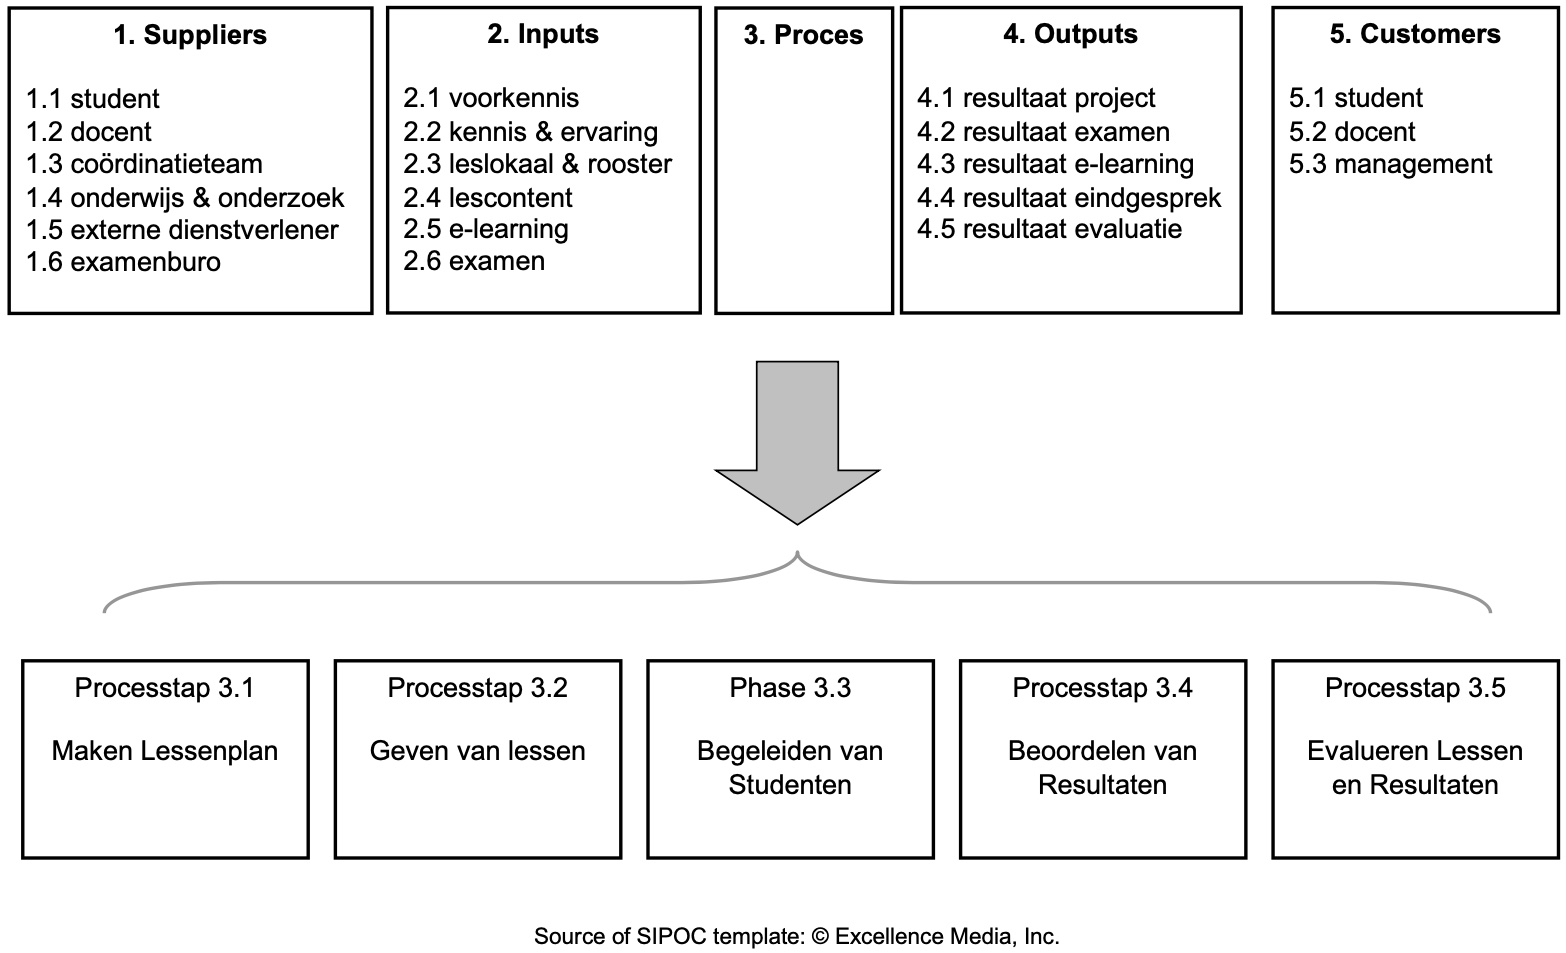
\includegraphics{./static/onderwijs_geven.jpg}

}

\caption{Onderwijsuitvoering}

\end{figure}%

Ter algemene toelichting:

\begin{itemize}
\tightlist
\item
  Het coördinatieteam zorgt ondermeer voor het samenstellen van het
  rooster.
\item
  Onderwijs \& onderzoek ondersteunt o.a. bij de inrichting en het
  gebruik van het LMS\footnote{Learning Management System, in het geval
    van de HvA het programma Brightspace.}.
\item
  De externe dienstverlener is in dit geval Skoledo waar de studenten de
  e-learnings volgen.
\item
  Het examenburo verzorgt de logistiek rondom de afname van examens.
\item
  Onder management wordt hier verstaan het hoofd van de opleiding
  Finance \& Control.
\end{itemize}

\newpage

\subsection{VOC-CTQ}\label{voc-ctq}

De Voice of the Customer, is de klantenvraag waardoor het project
geïnitieerd is. In dit project is het de Voice of the Business aangezien
de vraag (of opdracht) afkomstig is van de HvA academy, het interne
opleidingsinstituut van de HvA.\\
In de VOB-CTQ hieronder wordt verwezen naar drie termen uit de taxonomie
van Bloom: onthouden, toepassen en reproduceren. De taxonomie van Bloom
is een referentie waarnaar, binnen de HvA, regelmatig wordt verwezen. In
de taxonomie worden zes nivo's van leren onderscheiden. Omdat het
onderwerp van dit project een module is uit jaar 2, worden alleen de
onderste drie nivo's van de taxonomie benoemd.

\begin{figure}

\centering{

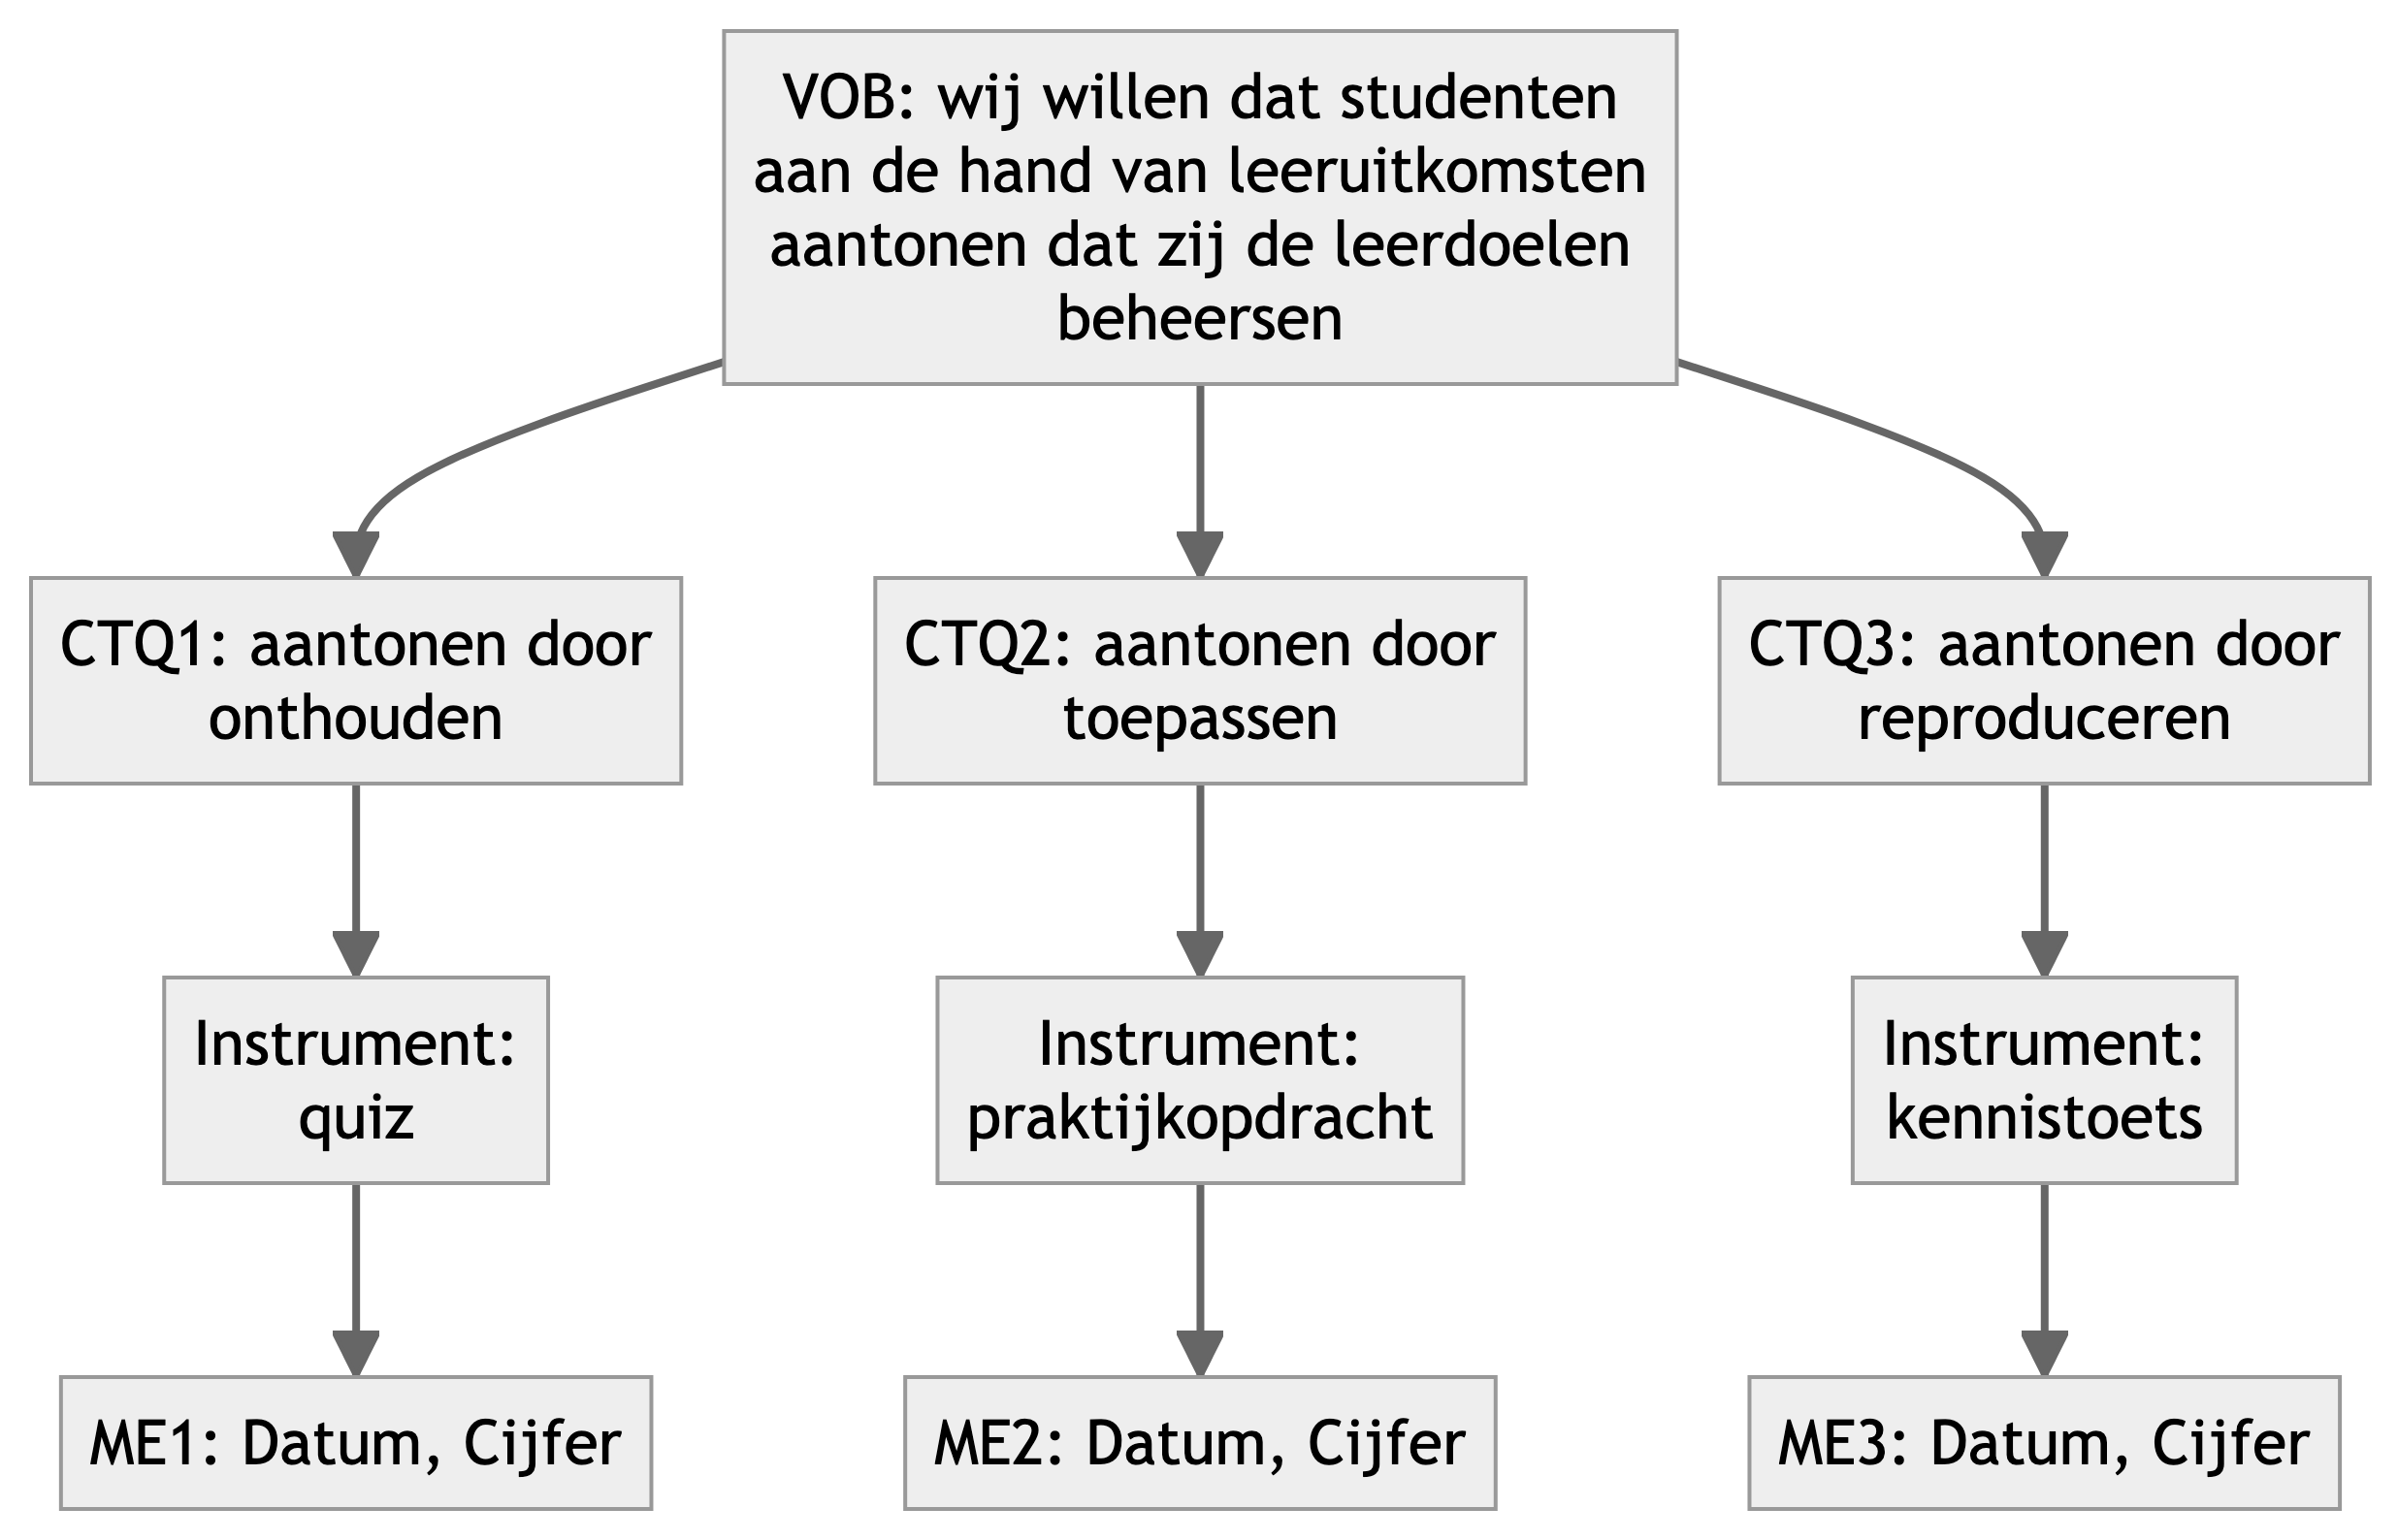
\includegraphics[width=6.45in,height=4.14in]{1_definitie_fase_files/figure-latex/mermaid-figure-1.png}

}

\caption{\label{fig-voc-ctq}Voice of the Business}

\end{figure}%

Waarschijnlijke toekomstige verbeteringen:

\begin{enumerate}
\def\labelenumi{\arabic{enumi}.}
\tightlist
\item
  In deze versie van de VOB-CTQ staan drie meetinstrumenten (quiz,
  praktijkopdracht, kennistoets) genoemd. In een latere versie wordt het
  instrument ``assessment'' daaraan toegevoegd en zullen de instrumenten
  (dan vier) verplaatst worden naar de meetfase.
\item
  In deze versie van de VOB-CTQ staan de meetbare eenheden (ME) appart
  genoemd per CTQ. In een latere versie kunnen alle drie de CTQ's
  verwijzen naar twee meetbare eenheden: datum en cijfer.
\item
  Er dient nog een CTQ over ``volgordelijkheid'' te worden toegevoegd.
  Hiervoor dient de VOB nog te worden aangepast (met een statement over
  effectiviteit).
\end{enumerate}

\newpage

\subsection{Prestatie indicator}\label{prestatie-indicator}

De grafische prestatie indicator dient weer te geven wat:

\begin{itemize}
\tightlist
\item
  de ideale doorlooptijd van de e-learnings is
\item
  wat de feitelijke doorlooptijd van de e-learnings is.
\end{itemize}

Voor de ideale doorlooptijd van de e-learnings is de studiegids leidend
in combinatie met de daadwerkelijke opdrachten op Brightspace. Voorwat
betreft de feitelijke doorlooptijd van de e-learnings is de rapportage
van Skoledo leidend.

\textsubscript{Source:
\href{https://jan-ru.github.io/lss_greenbelt/1_definitie_fase.qmd.html}{Article
Notebook}}

\begin{figure}[H]

\centering{

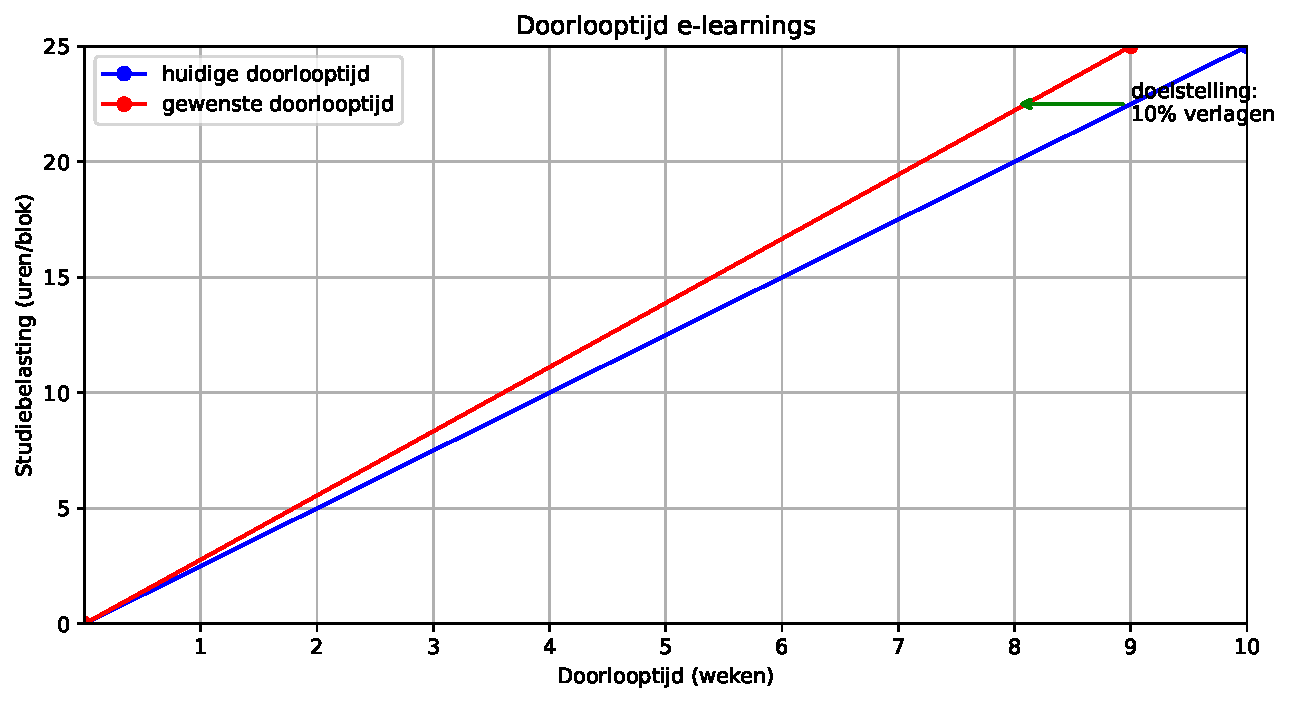
\includegraphics{1_definitie_fase_files/figure-pdf/fig-lineplot-output-1.pdf}

}

\caption{\label{fig-lineplot}A line plot showing progress on the
e-learnings}

\end{figure}%

\textsubscript{Source:
\href{https://jan-ru.github.io/lss_greenbelt/1_definitie_fase.qmd.html}{Article
Notebook}}

De totale studiebelasting voor de e-learnings is circa 25 uur (zie
bijlage B). De duur van een blok is 10 weken.

Vooralsnog bestaat de grafische prestatie indicator uit twee fictieve
lijnen.

\begin{itemize}
\tightlist
\item
  De {blauwe} lijn is bedoeld de huidige ideale doorlooptijd van de
  e-learnings weer te geven.
\item
  De {rode} lijn is bedoeld de nieuwe ideale doorlooptijd van de
  e-learnings weer te geven (10\% korter).
\end{itemize}

De twee lijnen zullen worden aangepast zodra de studiegids en het
programma in detail gelezen zijn. Naast de oude en nieuwe ideale
doorlooptijd wordt in het resultaten hoofdstuk ook de feitelijke
doorlooptijd getoond.

\textsubscript{Source:
\href{https://jan-ru.github.io/lss_greenbelt/1_definitie_fase.qmd.html}{Article
Notebook}}



\end{document}
